\subsection{The Selection of Cities}
%Section \ref{sec:eceexperiences} shows that the childcare systems within and outside Reggio Emilia share the Reggio Approach components to varying degrees. Because other childcare options may be similar to the Reggio Approach to some extent and may have their own high-quality components, it is difficult to evaluate the clean effects of the Reggio Approach. 
Our survey data collection is designed to evaluate the impact of the Reggio Approach on life-time social and economic outcomes comparing it to other early childhood programs that might share similar components. Note that our comparison is not to determine whether the Reggio Approach is of higher or lower quality relative to other programs, but rather to understand how these programs that vary across school types, cities, and over time might have differential impact of life-time outcomes.

We collect data on five cohorts of individuals born and raised in Reggio Emilia, Parma, and Padova. Parma and Padova have been chosen in addition to Reggio Emilia to represent appropriate controls: they are close enough to Reggio Emilia in terms of size, geographic, demographic, and socio-economic structure, but they did not experience its unique approach to early childhood education.\footnote{Other Italian cities were taken into consideration, notably Brescia, Livorno, Modena, Perugia, Piacenza, Prato, and Ravenna. Parma and Padova were the two cities that best fulfilled our comparability and sample requirements.} For example, Reggio Emilia has a population of roughly 173,000, Parma of 188,000, and Padova of 210,000 in 2013.\footnote{The population size in December 2013 was 172,525 in Reggio Emilia, 187,938 in Parma, and 209,678 in Padova. Source: ISTAT, \url{http://www.demo.istat.it/}} Also their economic resources are comparable: Reggio Emilia has an average per-capita income of 25,226 euros, Parma of 28,437, and Padova of 29,915 in 2011.\footnote{Source: Finance Minister, taxable income for 2011.} 
%See \url{http://www.comuni-italiani.it/statistiche/redditir2011.html}
Even more importantly, these three cities face analogous fertility dynamics and, consequently, potential demand for child-care services. The three cities had a very similar number of births from both Italians and immigrants in the past decade. Parma is a neighboring city 30 km to the west of Reggio Emilia, it belongs to the same administrative region of Emilia-Romagna, and shares with Reggio a common background that forged the city's political and economic system, and shaped its culture and social capital; yet Parma has witnessed a different approach to public investment in early childhood education. On the contrary, Padova lies 150 km away from Reggio Emilia, in the richer north-eastern region of Veneto, and was more influenced by the history and culture of Venice. Yet, Padova, just as Reggio Emilia, is a middle-size Italian city with a thriving migrant population, facing similar political and economic issues, with a different social background but similar resources which can be devoted to early childhood education.

Figure \ref{fig:enrollment} explores the similarities and difference in enrollment statistics in three cities. Note that enrollment data is not available for Parma except for the year 2010. It is shown that Padova has the highest rate of attending preschool. It is also shown that Reggio Emilia and Padova observed the increase in preschool enrollment; from the 1990s, almost all children of age 3-5 are enrolled in preschool. The figures also show that the percentage of enrollment in municipal preschools increased during the 1970s and the 1980s in Reggio Emilia and Padova, but decreased after the 1990s in Reggio Emilia. The percentage enrolled in state preschools increased over time in both Reggio Emilia and Padova. In contrast, the percentage enrolled in private preschools decreased over time in Reggio Emilia and Padova. For Parma, the enrollment statistics in 2010 are similar to those of Reggio Emilia. 
 
\begin{figure}[H]
      \centering
        \begin{subfigure}[t]{0.49\textwidth}
          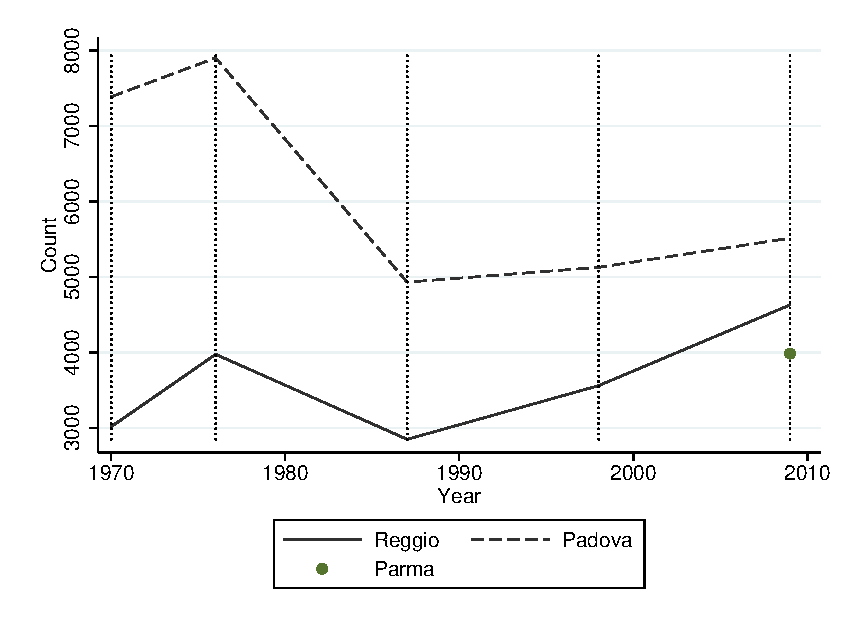
\includegraphics[width=\textwidth]{../../output/image/enroll_num_graph.eps}       
\caption{Num. of Children Enrolled in Preschool}        
        \end{subfigure}
        \begin{subfigure}[t]{0.49\textwidth}
          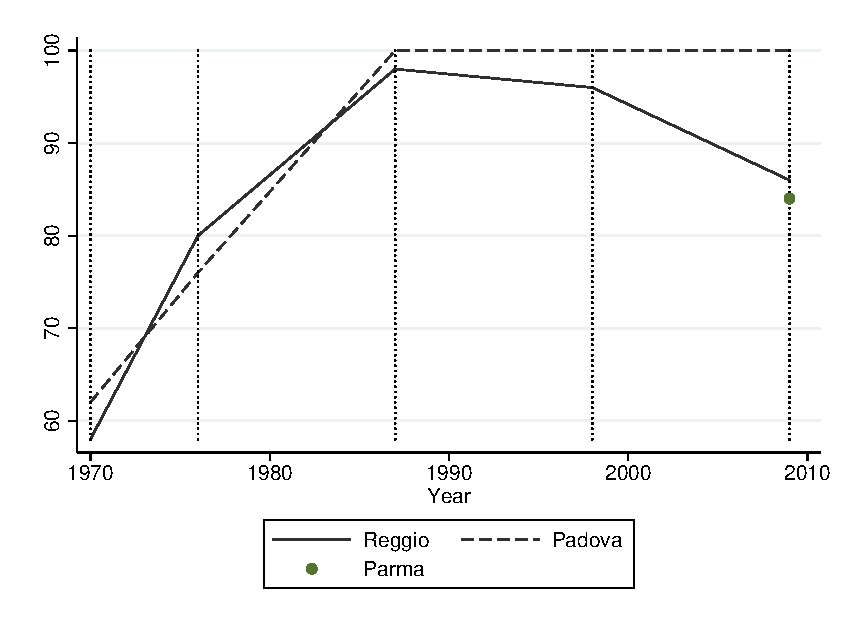
\includegraphics[width=\textwidth]{../../output/image/enroll_per_graph.eps}       
 \caption{Percentage of Ages 3-5 Enrolled in Preschool}        
        \end{subfigure}
        \begin{subfigure}[t]{0.49\textwidth}
          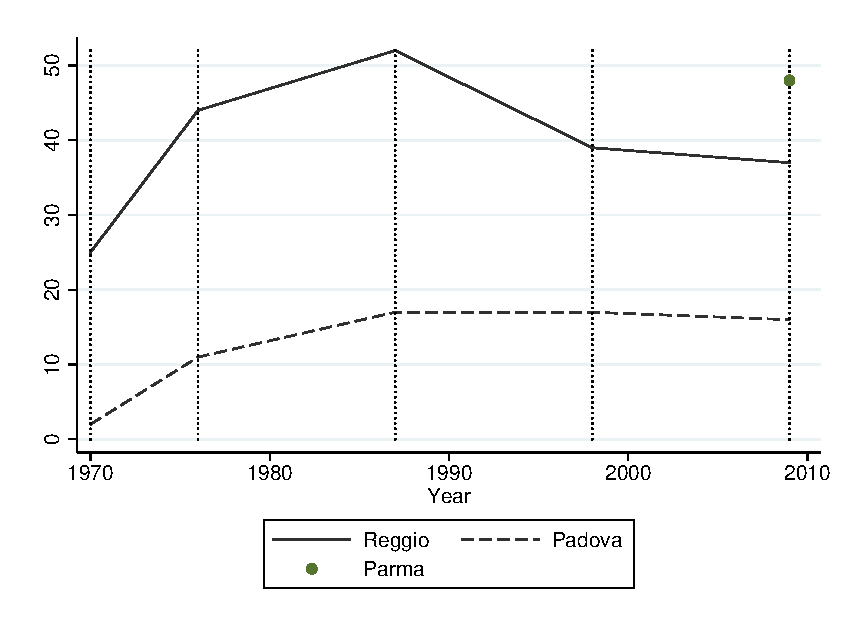
\includegraphics[width=\textwidth]{../../output/image/enroll_per_muni_graph.eps} 
        \caption{Percentage of Enrollment in Municipal Preschool}        
        \end{subfigure}
        \begin{subfigure}[t]{0.49\textwidth}
          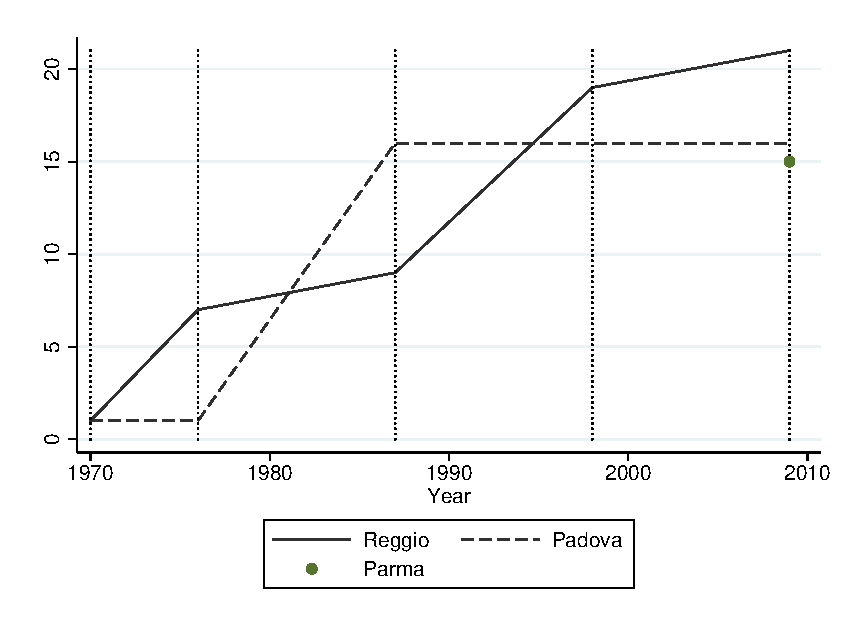
\includegraphics[width=\textwidth]{../../output/image/enroll_per_stat_graph.eps}
            \caption{Percentage of Enrollment in State Preschool}       
        \end{subfigure}
      \begin{subfigure}[ht]{0.48\textwidth}
        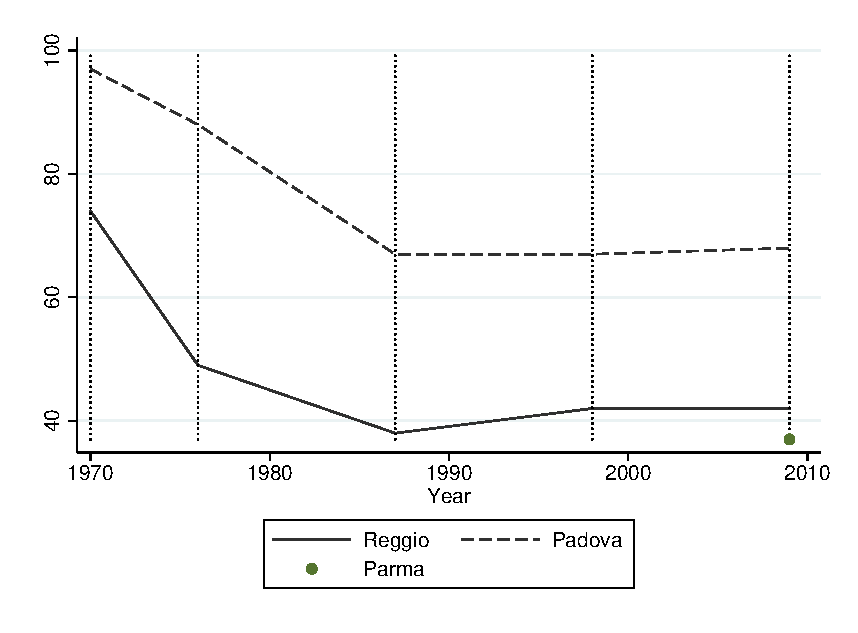
\includegraphics[width=\textwidth]{../../output/image/enroll_per_priv_graph.eps}
        \caption{Percentage of Enrollment in Private Preschool}
        \label{fig:large}
      \end{subfigure}
      \caption{Enrollment Statistics}  \label{fig:enrollment}
    \end{figure}


\subsection{The Survey Data Collection}

Respondents were sampled from the population registries of the cities based on their year of birth, in order to have a sample of children right after preschool age, of adolescents about to finish high-school, and adults who were in their 30s, 40s and 50s. The sample was then restricted to those individuals living in the same city in which they were raised. All cohorts, except the youngest one, are restricted to individuals who are Italian citizens. In contrast, the youngest cohort includes an oversampling of immigrant children.\footnote{In the adult cohorts there was no immigrant who was preschool age in the same school in which they live. In the adolescent cohort, the number was immigrant born was extremely small.} The sample from Reggio Emilia, across all cohorts, includes an oversampling of those who attended municipal schools, as this is considered the treatment group.

Of the reference sample, 7,109 individuals were randomly selected. Of these, 4,019 completed interviews, resulting in a response rate of 56.5\%. Table~\ref{tab:sample-city-cohort} provides an overview of the birth years for the different cohorts and the counts of the full sample.
\begin{table}[H]
\centering
\begin{threeparttable}
	\caption{Description of the Full Sample by Cohort and City}\label{tab:sample-city-cohort}
	\begin{tabular}{l c c c c c c}
\toprule
Cohort & Birth year(s) & Age at interview & \mc{4}{c}{Count} \\
\cmidrule{4-7}
 & 		&						& Reggio Emilia & Parma & Padova & \textbf{Total} \\
\midrule
\textbf{Children} &  &  &  & &  &  \\ 
\quad Italians & 2006 & 6 & 311 & 291& 278 & 880 \\
\quad Migrants & 2006 & 6 & 110 & 58 & 113 & 281 \\
\textbf{Adolescents} & 1994 & 19 & 300 & 254 & 282 & 836 \\
\textbf{Adults 30s} & 1980-1981 & 32 & 280 & 251 & 251 & 782 \\
\textbf{Adults 40s} & 1969-1970 & 43 & 285 & 254 & 252 & 791 \\
\textbf{Adults 50s} & 1954-1959 & 54-60 & 200 & 103 & 146 & 449 \\
\midrule
\textbf{Total}	& 				& & 1,486 & 1,211 & 1,322 & 4,019 \\
\bottomrule
\end{tabular}
\begin{tablenotes}
\footnotesize
Note: This table presents the number of individuals in the full sample. The age at interview is an approximation given there is some variation in the interview date and birth year within each cohort. In analysis, we combine the Italian and migrant subsamples of the child cohort and control for migrant status.
\end{tablenotes}
\end{threeparttable}
\end{table}

Table~\ref{tab:sample} provides a detailed tabulation of the sample by city, cohort, and school type. It shows that the number of people who do not attend any preschool decreases over time. Whereas the majority of individuals from the age-50 cohort did not attend any preschool, there are few such cases in the child and adolescent cohorts. Table \ref{tab:sample} also shows that the proportion of individual attending municipal preschools is higher in Reggio Emilia than in the other cities.\footnote{This is due to the construction of the sample.} Note that the Reggio Approach preschools were not available for the age-50 cohort, as demonstrated in Table \ref{tab:itc-pre} and Table \ref{tab:sample}. 

\begin{table}[H]
\centering
\scalebox{0.85}{
\begin{threeparttable}
	\caption{Tabulation of Preschool Attendence by Cohort, City, and School Type}\label{tab:sample}
	\begin{tabular}{l*{8}{c}}
\toprule
	&	\mc{7}{c}{Reggio Emilia: 1,486}													\\	\midrule
	&	None	&	Muni	&	State	&	Reli	&	Priv	&	Muni-Affi	&	Other	\\	\midrule
Children	&	2	&	159	&	44	&	92	&	5	&	7	&	1	\\	
Migrants	&	4	&	47	&	38	&	14	&	1	&	3	&	1	\\	
Adolescents	&	7	&	151	&	22	&	98	&	6	&	13	&	0	\\	
Adults 30s	&	57	&	138	&	31	&	40	&	1	&	4	&	8	\\	
Adults 40s	&	80	&	87	&	14	&	52	&	5	&	1	&	43	\\	
Adults 50s	&	147	&	0	&	0	&	29	&	2	&	0	&	20	\\	\midrule
	&	\mc{7}{c}{ Parma: 1,211}													\\	\midrule
	&	None	&	Muni	&	State	&	Reli	&	Priv	&	Muni-Affi	&	Other	\\	\midrule
Children	&	5	&	105	&	42	&	74	&	8	&	52	&	0	\\	
Migrants	&	4	&	25	&	12	&	3	&	6	&	7	&	0	\\	
Adolescents	&	4	&	100	&	52	&	77	&	6	&	5	&	2	\\	
Adults 30s	&	44	&	85	&	56	&	51	&	5	&	4	&	3	\\	
Adults 40s	&	116	&	0	&	0	&	55	&	1	&	4	&	73	\\	
Adults 50s	&	72	&	0	&	0	&	11	&	0	&	10	&	9	\\	\midrule
	&	\mc{7}{c}{Padova: 1,322}													\\	\midrule
	&	None	&	Muni	&	State	&	Reli	&	Priv	&	Muni-Affi	&	Other	\\	\midrule
Children	&	2	&	58	&	45	&	141	&	12	&	19	&	0	\\	
Migrants	&	5	&	33	&	46	&	23	&	1	&	0	&	4	\\	
Adolescents	&	1	&	84	&	46	&	132	&	6	&	7	&	2	\\	
Adults 30s	&	47	&	27	&	27	&	140	&	1	&	7	&	0	\\	
Adults 40s	&	75	&	0	&	0	&	126	&	0	&	10	&	39	\\	
Adults 50s	&	57	&	0	&	0	&	72	&	2	&	6	&	3	\\	

\bottomrule
\end{tabular}


\begin{tablenotes}
Note: This table shows the sample size by city, cohort, and school type. We separate migrants and children for clarity in this table even though they are in the same birth cohort (year of birth: 2006). None: no preschool; Muni.: municipal preschool;  State: state preschool; Relig.: religious preschool; Priv.: private preschool. Muni-Affi: municipal-affiliated preschool; Other: uncategorized preschool.
\end{tablenotes}
\end{threeparttable}
}
\end{table}

The structure of the cohorts allows us to study the effects of the Reggio Approach at different points throughout the life cycle. The children in the youngest cohort were interviewed when they entered primary school, the adolescent cohort when they ended compulsory schooling, and the adult cohorts capture different points of adulthood to measure key outcomes such as engagement in the labor market, health, and family decisions. This cohort structure also allows us to evaluate the Reggio Approach compared to the alternative early childhood experiences over time.

Restricting the sample to individuals living in the same city in which they were raised is necessary in order to compare individuals who had the \textit{opportunity} to attend the different types of preschool. Due to the the municipal structure of the population registries, it is not feasible to sample all individuals born in Reggio Emilia, Parma or Padova and now living in other cities or abroad. If the Reggio Approach has a treatment effect on migration out of Reggio Emilia, then our sample might oversample individuals with characteristics that are not predictive of emigration. Table~\ref{tab:immigration} presents the proportion of people who were born in Italy, of Italian citizenship, and then still resident in that town of birth, out of the total number of names given by the population registries. For all cohorts, the immigration rates are very similar for all three cities. This reinforces our choice of treatment and control cities, which share a similar economic and labor market history. Nonetheless, it is worth noting that embedded in our sample selection is the potential bias due to the fact that one of the effects of preschool might be a higher propensity to emigrate. 

\begin{table}[H]
\centering
\begin{threeparttable}
	\caption{Percentage of People Living in the Same City Since Birth}\label{tab:immigration}
	\begin{table}[ht!]
\caption{\textbf{Percentage of people living in the same city since birth, by cohort}}
\label{tab:SameCity}
\vspace{-5mm}
\begin{center}
\begin{tabular}{ l c c c c }
\hline\hline
\textbf{Cohort} & \textbf{Reggio (\%)} & \textbf{Parma (\%)} & \textbf{Padova (\%)} & \textbf{Total (\%)}\\
\hline
Italian Children born in 2006 (Cohort V)   & 61.3  & 70.2  & 65.1  & 65.2 \\[0.2em]
Adolescents born in 1994 (Cohort IV)       & 58.1  & 63.0  & 64.4  & 61.9 \\[0.2em]
Adults born in 1980-81 (Cohort III)        & 26.5  & 27.5  & 32.6  & 29.0 \\[0.2em]
Adults born in 1969-70 (Cohort II)         & 27.9  & 31.6  & 31.9  & 30.6 \\[0.2em]
Adults born in 1954-59 (Cohort I)          & 28.8  & 27.9  & 31.4  & 29.5 \\[0.2em]
\hline
\textit{Total}         & \textit{32.3\%}  & \textit{32.5\%}  & \textit{35.2\%} & \textit{33.5\%} \\
\hline
\end{tabular}
\end{center}
\footnotesize{{\bfseries Notes:} Reference sample who satisfied the selection criteria (born in the city of residence and of Italian citizenship) as a percentage of the total number of names given by the population registries, broken down by City and Cohort. Source: authors calculations on data provided by the population registries.}
\end{table}

\begin{tablenotes}
\footnotesize
Note: This table presents the percentage of people living in same city since birth. This  shows the reference sample who satified the selection criteria (born in the city of residence and of Italian citizenship) as a percentage of the total number of names given by the population registries.
\end{tablenotes}
\end{threeparttable}
\end{table}

%\subsection{The Questionnaire Design}

In order to allow us an evaluation of the potential effect of the Reggio Approach on a broad set of domains, we designed a questionnaire surveying various outcomes and dimensions of life success. Respondents were asked about family composition, fertility, labor force participation, income, schooling, cognitive ability, social and emotional skills, health and healthy habits, social capital, interpersonal ties, as well as attitudes on migrants. Three age-specific questionnaires were designed, piloted, and fielded: one for the Italian and immigrant child cohorts, one for the adolescent cohort, and one for the adult cohorts.\footnote{By means of a first pilot in the city of Bergamo with a sample from every cohort, and a second pilot in Reggio Emilia, Parma, and Padova on a subsample of adults, the questionnaires were tested and refined to the final version, which lasts approximately 40 minutes for the adults, and 1 hour for the children and the adolescents.}

%The child and adolescent questionnaires are further divided in two main parts: one answered by the caregiver, with questions about the child but also about herself and her family, and a second part answered directly by the child or adolescent. Two survey modes have been tested and piloted to achieve the optimal wording, timing, and length\footnote{By means of a first pilot in the city of Bergamo with a sample from every cohort, and a second pilot in Reggio Emilia, Parma, and Padova on a subsample of adults, the questionnaires were tested and refined to the final version, which lasts approximately 40 minutes for the adults, and 1 hour for the children and the adolescents.}: a face-to-face Computer Assisted Personal Interview (CAPI), and a Paper And Pencil Interview (PAPI), both of which are included in the sample data. Both contain exactly the same questions, but the CAPI is a survey mode intended particularly for the children and all those who agree to a face-to-face interview, while the PAPI is a survey mode targeted to those who prefer to take their time and answer questions on their own.

%The questionnaires are divided in different sections each addressing a specific domain of the
%respondent's life that could be influenced by early-life experiences. These
%domains can be classified into three broad categories: (1) demographic and
%socio-economic characteristics of the respondents; (2) mental, social, and
%emotional wellbeing; (3) attitudes toward themselves and society. In the
%following we describe each of them in turn.
%
%\subsubsection{Demographic and Socio-Economic Characteristics}
%
%The first part of the questionnaire gathers information on the demographic
%and socio-economic characteristics of the respondent's family in the
%following five domains: family composition, education, labor market,
%marriage, and fertility. Besides containing standard background information
%on the characteristics of each member of the household, this section asks
%extensive information on early-childhood education and family background.
%The respondents are asked about child care choices in the first six years of
%life, the name and address of any infant-toddler center and preschool
%attended, the age of attendance, and the reason behind these choices. For the younger cohorts, the caregivers are
%also asked about their own preschool experiences, and the children and
%adolescents about their attitudes towards school. Furthermore, adults and
%caregivers are surveyed about their relations with parents and grandparents,
%and about grandparents' involvement in child care. In the adult questionnaire, respondents are also asked about the social,
%economic, and religious background of their parents. 
%
%\subsubsection{Mental, Social, and Emotional Wellbeing}
%
%The Reggio Approach not only focuses on
%learning, but places a great emphasis on parental involvement in education
%and on the formation of health, emotional and behavioral skills, social
%capital, and cognitive ability. These skills are measured in the second part
%of the questionnaires with a variety of existing scales and tools as follows. First, caregivers and adults answer questions about
%parenting practices using the Home Observation Measurement for the
%Environment (HOME) scale, in order to evaluate the family environment of the
%younger cohorts, as well as to elicit the adults' attitudes to invest in
%their own children. Second, adolescents, caregivers, and adults are asked
%about the physical health and the healthy habits of themselves and of their
%children, including self-assessed health, eating and exercising habits, as well as drinking, smoking, and other risky
%behaviors. Third, the questionnaire measures various forms of
%socio-emotional skills and mental health conditions. Respondents are asked
%to fill in the Strength and Difficulties Questionnaire (SDQ)\footnote{SDQ is a brief behavioural screening questionnaire about 3-16 year olds. It inquires about (1) emotional symptoms, (2) conduct problems, (2) hyperactivity/inattention, (4) peer relationship problems, and (5) prosocial behavior.}, a short
%version of the Rotter Locus-of-Control Scale, the 10-item Center for
%Epidemiologic Studies Depression (CES-D) Scale, questions regarding
%satisfaction using Self-Anchoring Ladder \citep{Cantril_1965_BOOK_Pattern-Hum-Con}, and to report
%personal stress and time usage following the ISTAT-Indagine Multiscopo
%questions. Using age-appropriate scales with emoticons from the Child
%Outcome Rating Scale (CORS), children are asked about their happiness and
%satisfaction. Fourth, in the realm of social capital, adults and adolescents
%are asked questions about social networks, discrimination, friendship ties,
%religiosity, and political inclination. The children's questionnaire also
%contains questions regarding friendship, reciprocity, and sharing attitudes.
%Finally, at the very end of each questionnaire all the respondents take a
%nonverbal IQ test: a short version of the Raven
%Progressive Matrices. We modify all cognitive and noncognitive measures so that the higher value means more socially positive outcome.
%
%\subsubsection{Attitudes Towards Self and Society}
%
%The final category of questions focuses on the respondents' attitudes
%towards themselves and society, asking about four domains: their opinions
%about society, their level of trust and reciprocity, their future
%inclinations, and their attitudes towards immigration. Caregivers, adults,
%and adolescents are asked their opinions and satisfaction with the
%public services offered by the city, their thoughts on prohibition of
%alcohol and drugs, and their level of trust and reciprocity towards
%strangers.\footnote{%
%These same questions are used in the German Socio-Economic Panel (G-SOEP) %
%\url{www.diw.de/gsoep/}. The questions about trust
%were also asked to the caregivers.} Adults are also asked about their
%opinion on gender and family issues, while adolescents about their
%sentimental life. All these questions are asked because attending a Reggio Approach school could have
%shaped the way the respondents view the world around them. Adolescents and
%children also share information regarding future inclinations on career plan, marriage, and success in life. Finally, another unique feature of our questionnaires is the section that elicits the respondents' attitudes toward immigration. Adolescents, adults, and caregivers answer one of two sets of questions, according to their nationality: Italians are asked about their general opinion about immigration and their contact with foreigners; immigrants are asked about their experiences of integration within the city. Furthermore, the self-completion section of the questionnaire contains more straightforward questions about racism, immigration policy, and willingness to befriend or live next door to a foreigner.